\documentclass[10pt,a4paper,titlepage,oneside]{report}
\usepackage[utf8]{inputenc}
\usepackage[czech]{babel}

\usepackage{amsfonts}
\usepackage[IL2]{fontenc} 
\usepackage{graphicx}
\usepackage{epstopdf}
\usepackage{fancyhdr}
\usepackage{mathtools}
\usepackage{float}
\usepackage{color}
\usepackage{hyperref}
\hypersetup{
    colorlinks,
    citecolor=black,
    filecolor=black,
    linkcolor=black,
    urlcolor=black
}
\usepackage[justification=centering]{caption}


\newcommand{\HRule}{\rule{\linewidth}{0.5mm}}

\newcommand{\itab}[1]{\hspace{0em}\rlap{#1}}
\newcommand{\tab}[1]{\hspace{.2\textwidth}\rlap{#1}}
\newcommand{\red}[1]{\textbf{\rlap{\color{red}#1}}}

\usepackage[top=2.5cm, bottom=2.5cm, left=2.5cm, right=2.5cm]{geometry}
%\usepackage[a4paper]{geometry}

\providecommand{\e}[1]{\ensuremath{\times 10^{#1}}}

%------------------------------------------------------------------------------------
%------------------------------------------------------------------------------------
%------------------------------------------------------------------------------------
%------------------------------------------------------------------------------------

\begin{document}
\title{Realizace experimentů pro odhad parametrů dynamického modelu látky}
\author{Michal Neoral}
\date{\today{}}
\maketitle


%------------------------------------------------------------------------------------
%------------------------------------------------------------------------------------
%------------------------------------------------------------------------------------
%------------------------------------------------------------------------------------
%------------------------------------------------------------------------------------
%------------------------------------------------------------------------------------
%------------------------------------------------------------------------------------
%------------------------------------------------------------------------------------
%------------------------------------------------------------------------------------
%------------------------------------------------------------------------------------
%------------------------------------------------------------------------------------
%------------------------------------------------------------------------------------
%------------------------------------------------------------------------------------
%------------------------------------------------------------------------------------
%------------------------------------------------------------------------------------
%------------------------------------------------------------------------------------

\chapter{Úvod}
\label{chap:intro}



\section{O projektu}
\label{sec:about}
Tato práce je součástí mezinárodního projektu CloPeMa (Clothes Perception Manipulation). Tento dokument popisuje sběr dat a postup realizace experimentů pro odhad parametrů dynamického modelu textilie. Více informací o projektu CloPeMa na internetových stránkách projektu~\cite{projekt} a na wikipedii projektu~\cite{wiki} 
\\

\section{Popis pracoviště}
\label{sec:desription}

%V této části jsou popsány nejdůležitější části manipulátoru pro tento experiment.

\begin{figure}[H]
	\centering  	
  	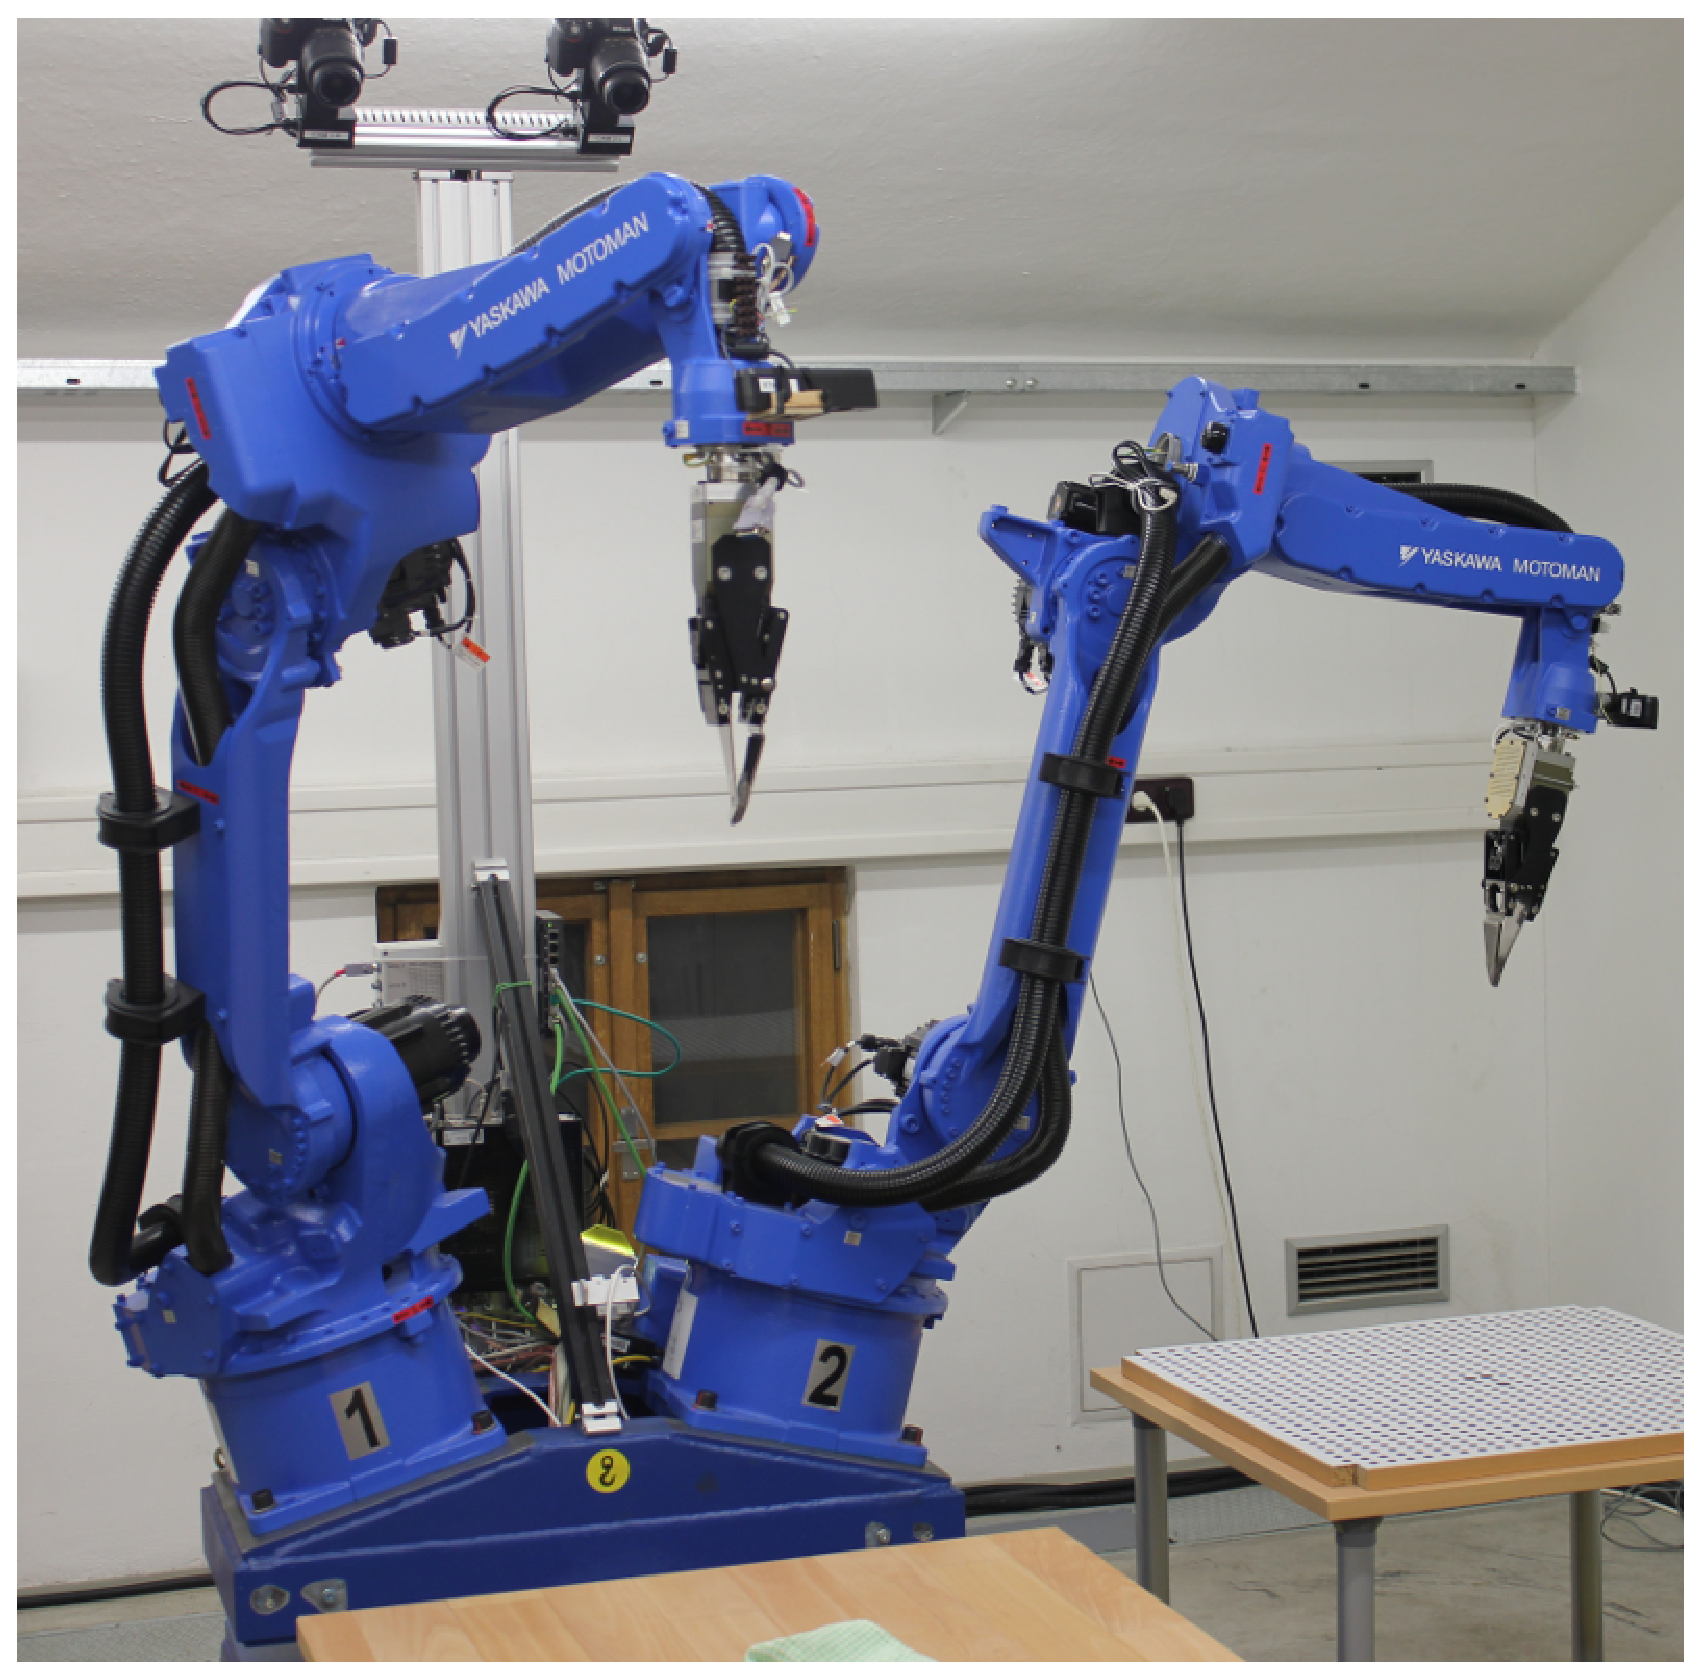
\includegraphics[height=7cm]{pictures/robotCTU.eps}
  	\caption[]{Manipulátor projektu CloPeMa umístěný na ČVUT v Praze.}
  	\label{fig:manipulatorCVUT}
\end{figure}

\subsection{Manipulátor}
\label{subsec:manipulator}

Základ manipulátoru tvoří dvě robotické paže Motoman~MA1400. Paže jedna je označena jako \verb|r1| (nebo se také objevuje \verb|R1|). Paže dvě je obdobně značena \verb|r2| (\verb|R2|). Paže \verb|r1| a \verb|r2| jsou umístěny na otočném stole. Otočný stůl se otáčí kolem osy označované jako \verb|Externí osa| (nebo také \verb|Ext.| případně jako \verb|13| osa). Umístění paží a otáčení \verb|Ext.| osy lze lépe vyčíst z obrázku~\ref{fig:motomanAndTable}. Každá paže manipulátoru má 6 os, okolo kterých je schopna se otáčet. Osy jsou dle výrobce označeny písmeny \verb|S|, \verb|L|, \verb|U|, \verb|R|, \verb|T| a \verb|B| (obrázek~\ref{fig:motomanAxis}). Toto označení nestačí a k písmennému názvu je třeba přiřadit i číslo paže, na které se tato osa nachází. Např.: osa \verb|S| nacházející se na paži \verb|r1| se bude nazývat \verb|S1| apod. Obdobně jako u označení paží se můžeme setkat i s použitím malých písmen.
\begin{figure}[H]
	\centering  	
  	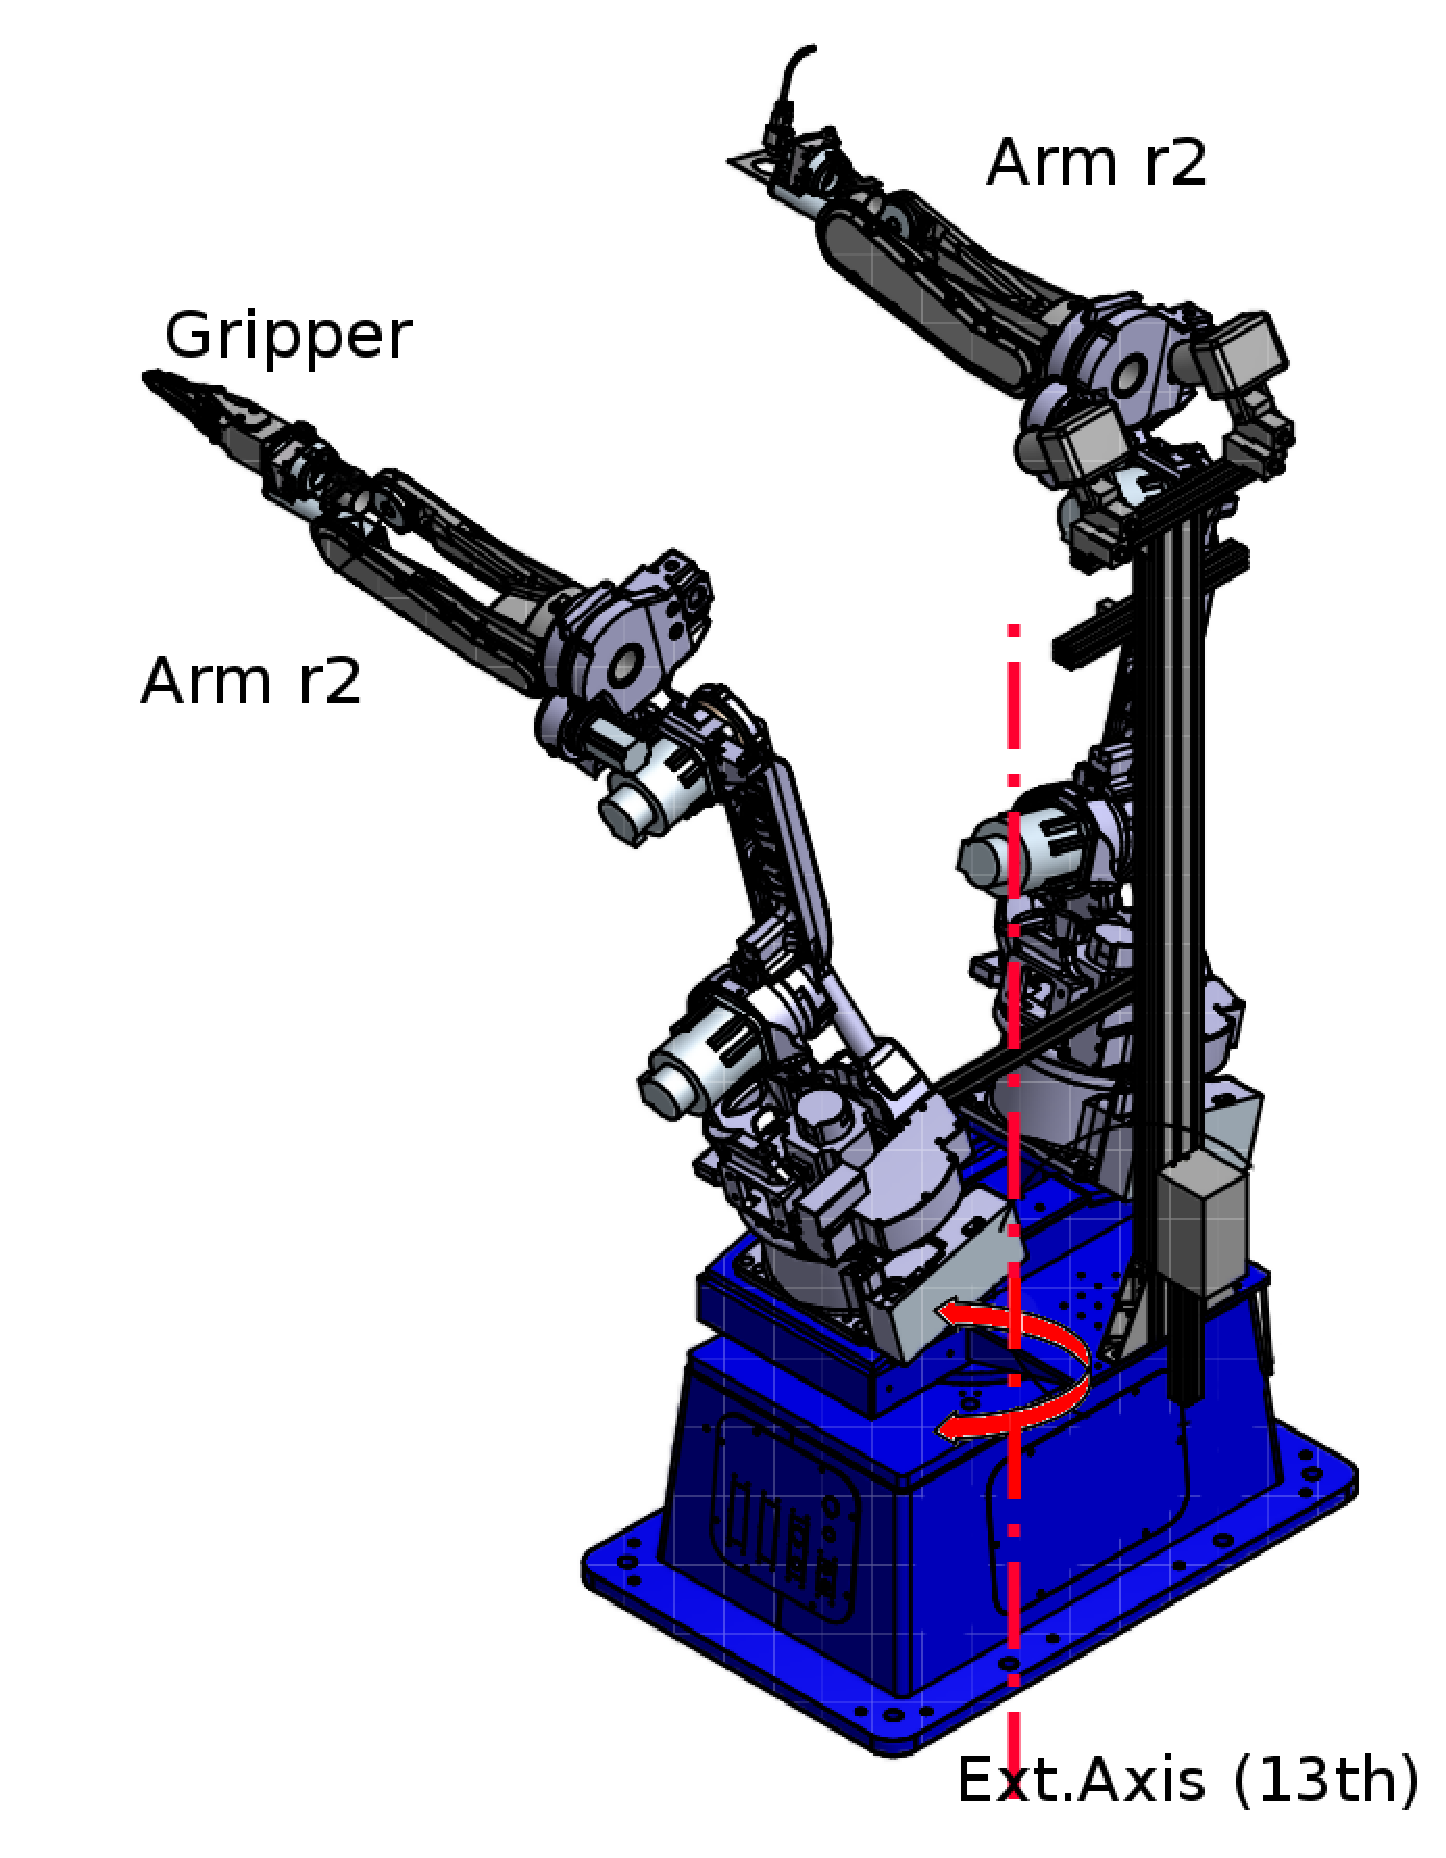
\includegraphics[height=7cm]{pictures/motomanCelek.eps}
  	\caption[]{Označení ramen a umístění Externí osy.\\
	Arm r1 - paže r1,
	Arm r2 - paže r2,
	Gripper - chapadlo,
	Ext.Axis (13th) - externí (třináctá) osa.	  	
  	}
  	\label{fig:motomanAndTable}
\end{figure}

\begin{figure}[H]
	\centering  	
  	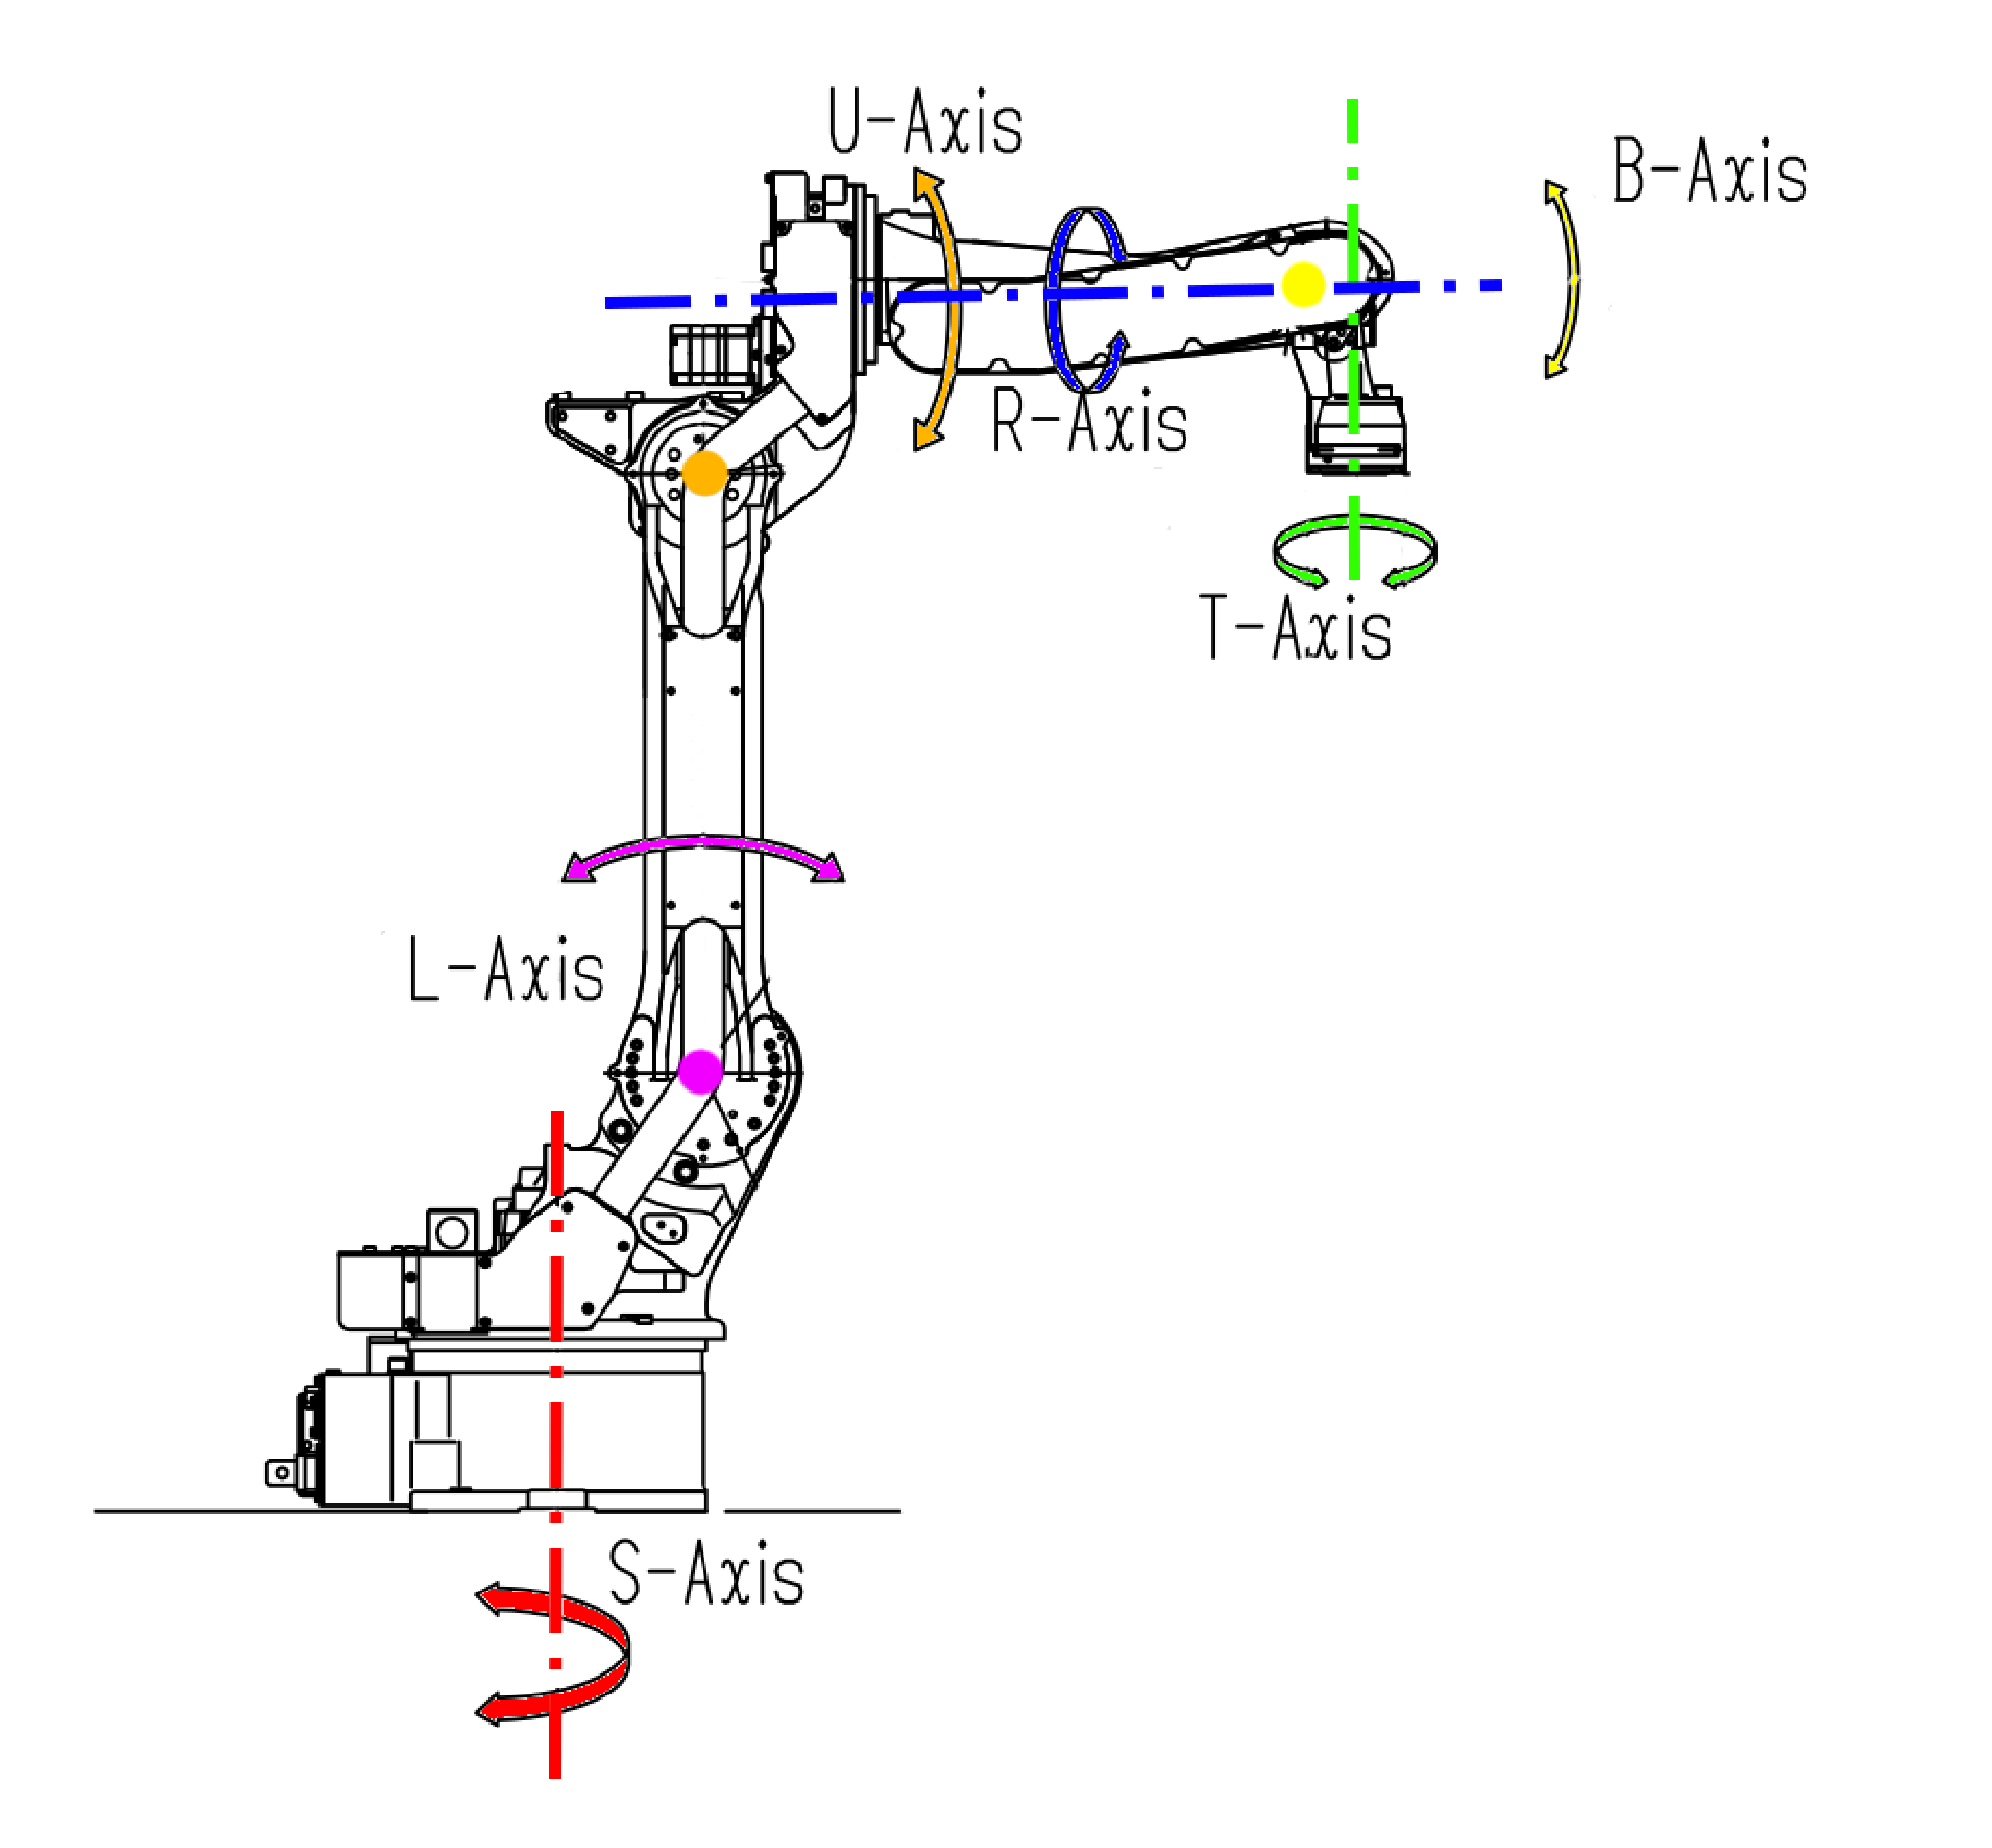
\includegraphics[height=8cm]{pictures/motomanMA1400axis.eps}
  	\caption[]{Popis os robotické paže Motoman MA1400.\\ 
  	S-Axis (červená) - osa S, 
  	L-Axis (fialová) - osa L, 
  	U-Axis (oranžová) - osa U, 
  	R-Axis (modrá) - osa R, 
  	B-Axis (žlutá) - osa B,
  	T-Axis (zelená) - osa T.}
  	\label{fig:motomanAxis}
\end{figure}

\subsection{Chapadlo}
\label{subsec:gripper}
Každá z paží \verb|r1| i \verb|r2| je zakončena elektricky ovládaným chapadlem obrázek~\ref{fig:gripper}. Chapadla slouží k držení textilií.

\begin{figure}[H]
	\centering  	
  	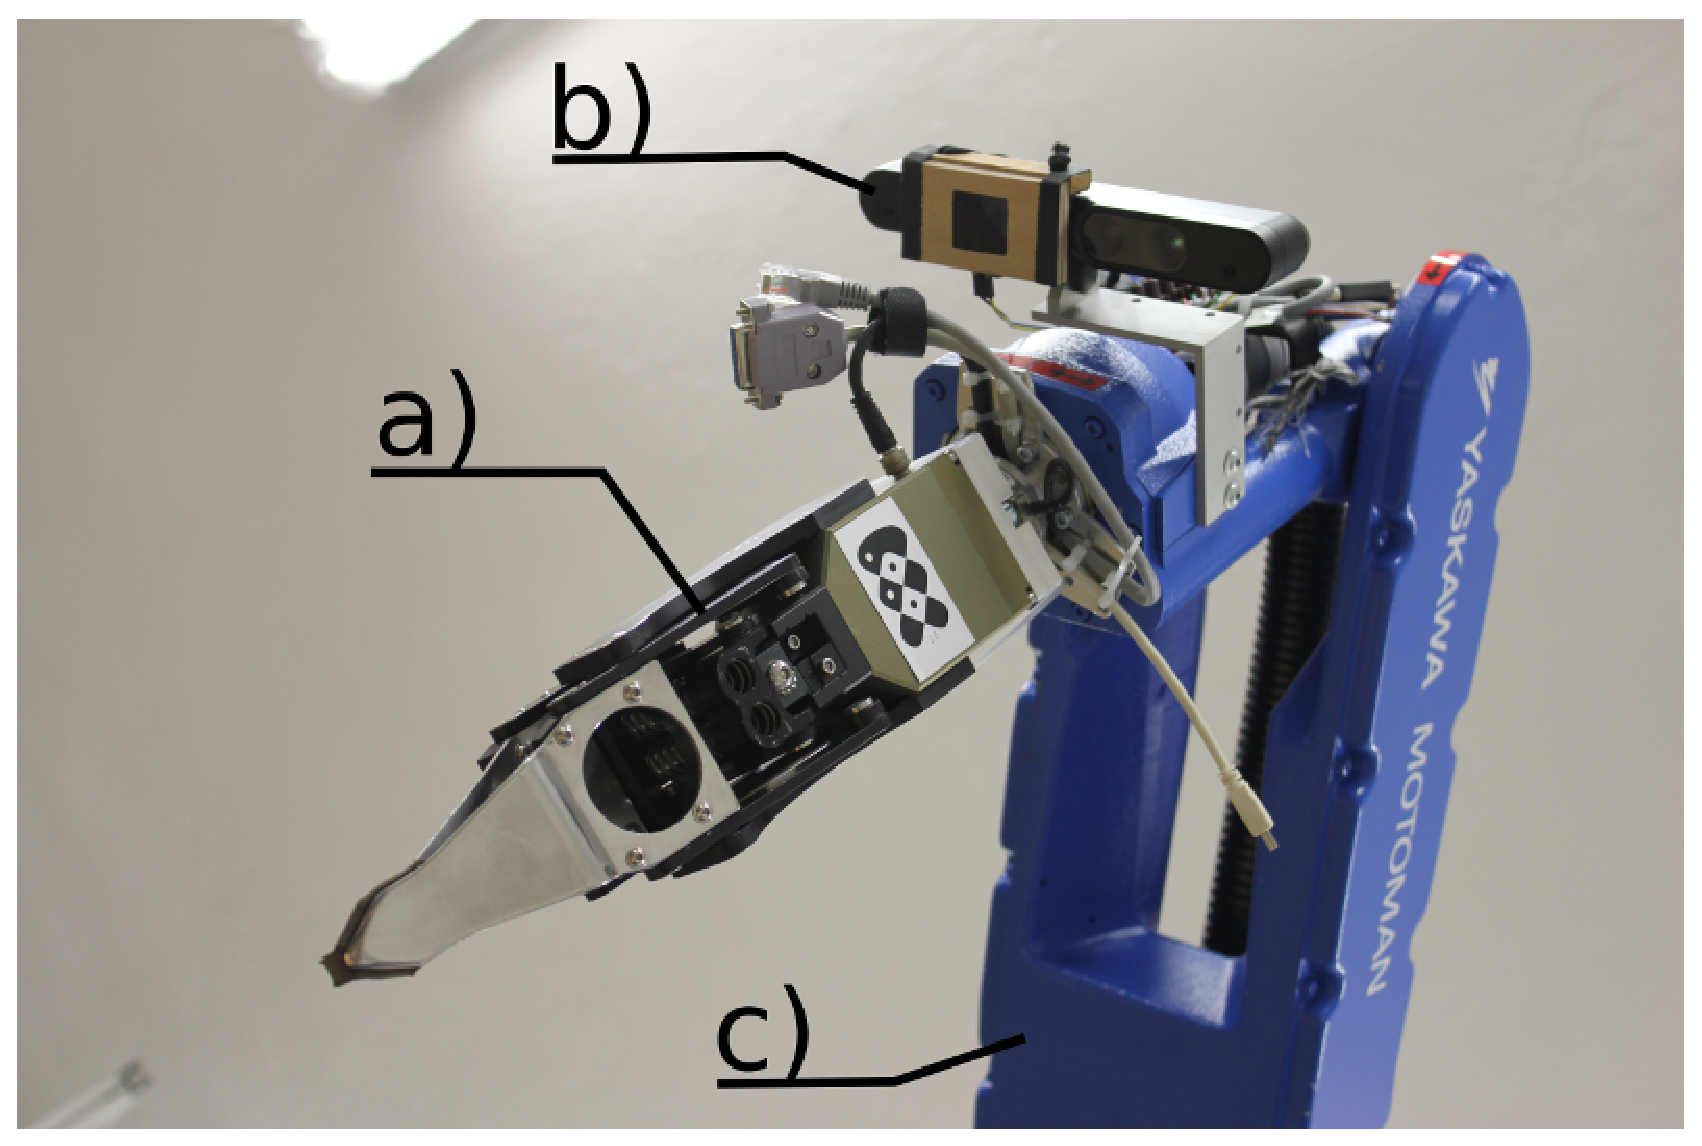
\includegraphics[height=7cm]{pictures/gripperXtion.eps}
  	\caption[]{Chapadlo.\\a) chapadlo, b) kamera Asus Xtion, c) konec paže, na které je chapadlo namontováno.	  	
  	}
  	\label{fig:gripper}
\end{figure}

\subsection{Kamera}
\label{subsec:camera}
Další důležitou částí manipulátoru je 3D~kamera Asus Xtion. Jedná se kameru, která je schopná zaznamenávat jak RGB snímky\footnote{Pro lepší manipulaci s RGB snímky je vhodné odfiltrovat pozadí. Způsobu provedení tohoto odfiltrování je naznačen v kapitolách~\ref{subsec:refRGB}~a~\ref{chap:matlab}.}, tak i hloubkovou mapu (\verb|depth|). Kamera namontovaná na paži \verb|r1| nese označení \verb|xtion1|, kamera namontovaná na paži \verb|r2| nese označení \verb|xtion2|. Umístění kamery je patrné na obrázku~\ref{fig:gripper}.\\
\\


%\begin{figure}[H]
%	\centering  	
%  	
\includegraphics[height=6cm]{pictures/xtion.eps}
%  	\caption[]{Asus Xtion namontovaný na ramenu manipulátoru.  	
%  	}
%  	\label{fig:xtion}
%\end{figure}

\noindent Tento popis obsahuje pouze vybrané části, které jsou důležité pro tento experiment. Podrobnější popis robota naleznete na Wikipedii projektu CloPeMa~\cite{wikiDes}. \\


\section{Požadavky na experiment}
\label{sec:experiment}
%Pro zjištění dat, které budou sloužit k odhadu parametrů dynamického modelu látky, jsme se rozhodli sledovat pohyb a chování textilie při %známém a opakovatelném pohybu. 
%Podle našeho názoru máme dvě možnosti snímání pohybu.
%Navrhněte metodu měření a získání matematických příznaků, které budou použity pro odhad parametrů dynamického fyzikálního modelu látky.
Požadavkem na experiment je získání matematických příznaků, podle kterých by se daly odhadnout parametry dynamického fyzikálního modelu látky. Tyto příznaky chceme určit na základě sledování pohybu visící látky. Pohyb visící látky bude vyvolán pohybem chapadla manipulátoru, které látku drží.\\ Na základě senzorů, které máme k dispozici, jsme si zvolili:
\begin{itemize}
\item nejjednodušeji pohyb, o kterém si myslíme, že by nám mohl poskytnout potřebná data k získání parametrů dynamického modelu látky. Tímto pohybem je pohyb látky v rovině, ideálně vybuzený pohybem chapadla s látkou po přímce (úsečce). 
\item dva typy sledování tohoto pohybu:
	\begin{itemize}
		\item Standardní RGB kamerou sledujeme siluetu, případně samotnou látku proti stálému pozadí při pohybu \textbf{kolmo k optické ose}.
		\item Senzorem snímající hloubkovou mapu sledujeme látku při pohybu \textbf{podél optické osy}.
		\end{itemize}
\end{itemize}


%\subsection*{Vodorovný pohyb známé délky - kolmo k optické ose.}
%Standardní kamerou sledujeme siluetu, případně samotnou látku proti stálému pozadí při pohybu \textbf{kolmo k optické ose}.
%
%\subsection*{Vodorovný pohyb známé délky - podél optické osy.}
%Při tomto pohybu by standardní kamera viděla jen vzdalující se (přibližující se) siluetu, proto použijeme hloubkovou mapu.





%------------------------------------------------------------------------------------
%------------------------------------------------------------------------------------
%------------------------------------------------------------------------------------
%------------------------------------------------------------------------------------
%------------------------------------------------------------------------------------
%------------------------------------------------------------------------------------
%------------------------------------------------------------------------------------
%------------------------------------------------------------------------------------
%------------------------------------------------------------------------------------
%------------------------------------------------------------------------------------
%------------------------------------------------------------------------------------
%------------------------------------------------------------------------------------
%------------------------------------------------------------------------------------
%------------------------------------------------------------------------------------
%------------------------------------------------------------------------------------
%------------------------------------------------------------------------------------

\chapter{Způsob pořízení dat}
\label{chap:proveData}
\section{Realizace}
Už při prvních pokusech jsme zjistili, že dynamika manipulátoru není natolik rychlá, aby s ním bylo možné provádět požadovaný pohyb  chapadlem s látkou po úsečce potřebnou rychlostí (kapitola~\ref{sec:experiment}). Je ovšem možné dosáhnou potřebné rychlosti, jestliže pohyb bude vycházet pouze z jednoho kloubu. Proto jsme s omezením robota museli pohyb chapadla s látkou realizovat tak, že pohyb chapadla po úsečce je aproximován pohybem chapadla po části kružnice. Dalším omezením je prostorové omezení a to takové, že není možné umístit kameru \verb|xtion| do pozice vhodné ke snímání RGB kamerou (tedy do pozice, kdy se chapadlo s látkou pohybuje kolmo k optické ose) a následně kameru \verb|xtion| přesunout do pozice vhodné ke snímání hloubkové mapy (tedy do pozice, kdy se chapadlo s látkou pohybuje podél optické osy). Toto omezení jsme vyřešili pomocí toho, že pozice kamery \verb|xtion|, tedy pozice paže s kamerou, je neměnná pro snímání záznamu RGB i pro snímání hloubkové mapy. Místo toho provede paže s textilií požadovaný pohyb chapadlem dvěma různými způsoby tak, aby byly splněny správné podmínky pro snímání jednotlivými senzory (kap.~\ref{sec:experiment} - pozice kolmo vs. podél optické osy).

\section{Výchozí pozice paží a celého manipulátoru}

\subsection{Paže s kamerou}
\label{sec:posArmR1}
Záznam je pořízen kamerou \verb|xtion1| namontovanou na paži \verb|r1|. Paže~\verb|r1| najede do polohy, ve které směřuje optická osa kamery \verb|xtion1| vodorovně. Zároveň je optická osa kamery \verb|xtion1| orientovaná směrem k paži \verb|r2| (obrázek \ref{fig:OptOsa}). \\
\begin{figure}[H]
	\centering  	
  	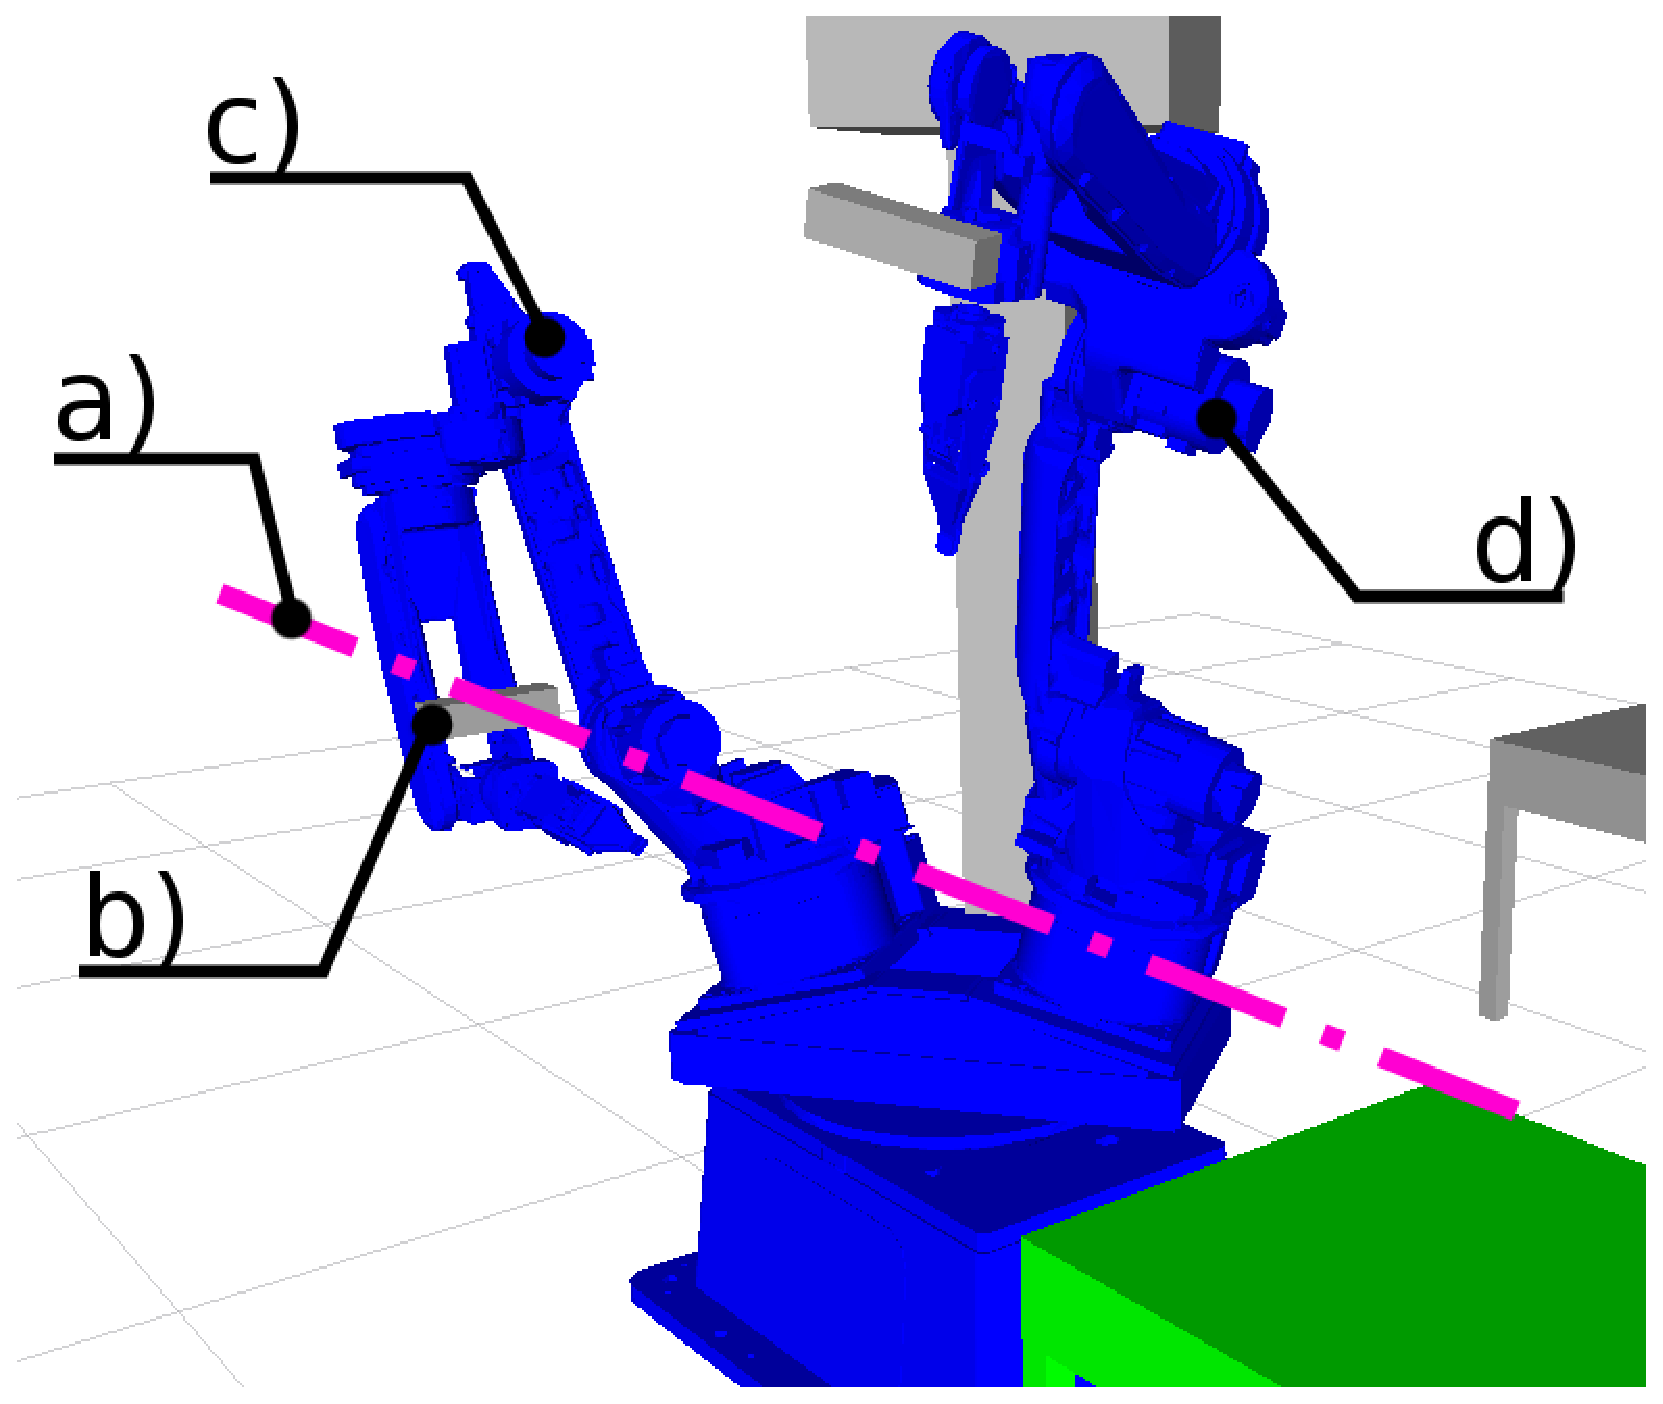
\includegraphics[height=7cm]{pictures/opOsa.eps}
  	\caption{Pozice paže s kamerou.\\a) Optická osa kamery xtion1, b) Kamera xtion1, c) paže r1, d) paže r2.}
  	\label{fig:OptOsa}
\end{figure}

\newpage
\subsection{Paže s textilií}
Textilie je držena pomocí chapadla namontovaného na paži \verb|r2|. Paže \verb|r2| nabývá dvou základních poloh. 
\subsubsection{Poloha pro měření}
Paže~\verb|r2| je v poloze, ve které je připravena k provedení experimentu. Paže \verb|r2| drží textilii v chapadle. Paže \verb|r2| je ve výšce, ve které je kamerou~\verb|xtion1| zaznamenána textilie. Paže~\verb|r2| je také v pozici, aby mohla provádět pohyb potřebný pro experiment (kapitola~\ref{sec:experiment} a kapitola~\ref{sec:moveArm}).

\subsubsection{Poloha pro referenční snímek}
\label{subsec:refRGB}
Tato poloha slouží k záznamu referenčního snímku pozadí, který slouží k odfiltrování pozadí z RGB snímků pro zlepšení přesnosti výsledků experimentu. Referenční snímek pozadí se nasnímá tak, že paže \verb|r2|, v jejímž chapadle je držena látka, změní pozici tak, aby byla zcela mimo oblast záznamu kamery~\verb|xtion1|. V této pozici se provede záznam pozadí a paže \verb|r2| s látkou se následně vrátí zpět do polohy pro měření. Více se odfiltrování pozadí budu věnovat v kapitole~\ref{subsec:matfiltr}.

\subsection{Otočení Ext.osy}
\verb|Externí osa| (osa č.: 13) je otočena tak, aby v pozadí snímané textilie bylo co nejméně rušivých předmětů. Nejlépe jednobarevný rovný povrch.

\section{Pohyby paží}
\label{sec:moveArm}

\subsection{Pohyb paže, aby se látka pohybovala kolmo k optické ose}
Paže \verb|r1| neprovádí žádný pohyb a je v poloze popsané v kapitole \ref{sec:posArmR1}. V chapadle paže \verb|r2| je držena textilie. Paže \verb|r2| provede požadovaný pohyb s touto textilií tak, že se otočí okolo osy \verb|B| o určitý úhel a vrátí se zpátky do výchozí polohy. Pro lepší popsání pohybu je pohyb naznačen i na obrázku \ref{fig:kolmoOptOsy}. Tento pohyb je vhodný ke snímání RGB kamerou.
\\
\begin{figure}[H]
	\centering  	
  	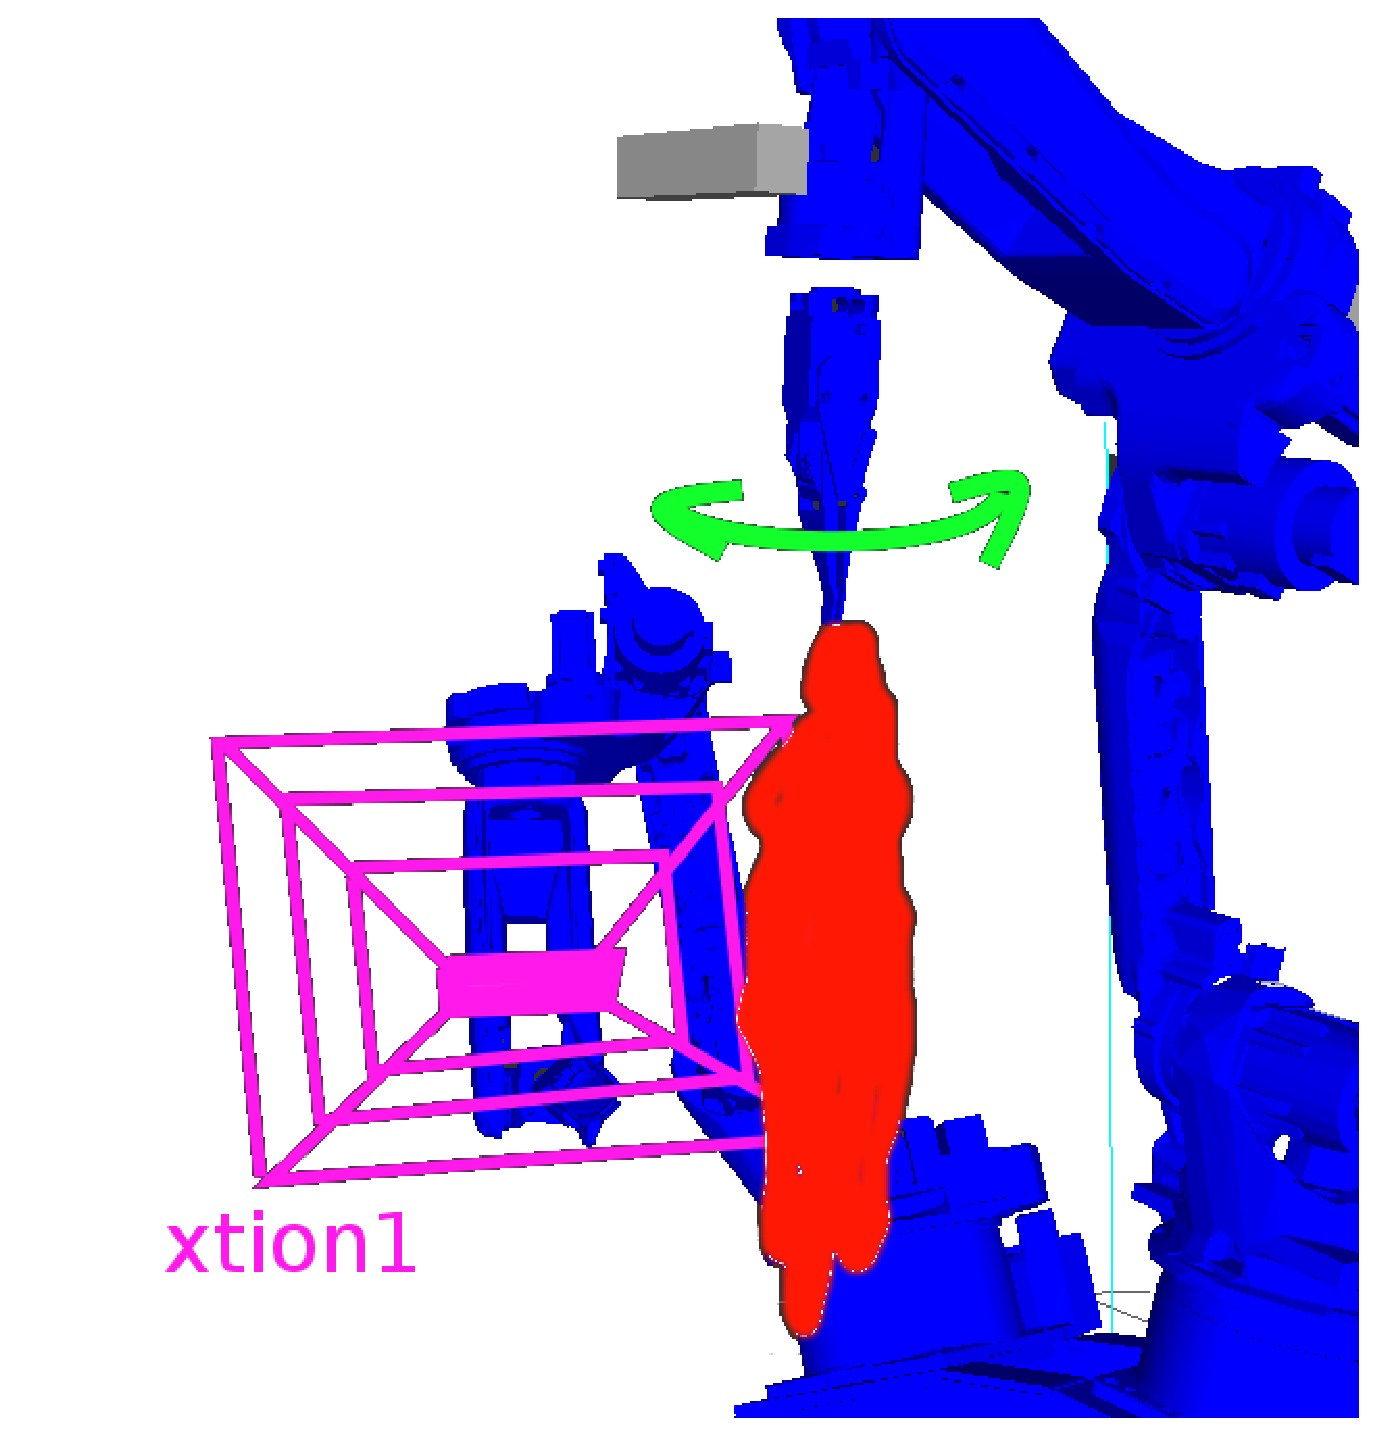
\includegraphics[height=7cm]{pictures/move1.eps}
  	\caption{Nastínění pohybů chapadla s textilií kolmo k optické ose.\\
  	a) naznačení zorného pole kamery xtion1, b) textilie, c) paže r1, d) paže r2.
  	}
  	\label{fig:kolmoOptOsy}
\end{figure}

\newpage
\subsection{Pohyb paže tak, aby se látka pohybovala podél optické osy}
Paže \verb|r1| neprovádí žádný pohyb a je v poloze popsané v kapitole \ref{sec:posArmR1}. V chapadle paže \verb|r2| je držena textilie. Paže \verb|r2| provede požadovaný pohyb s touto textilií tak, že se otočí okolo osy \verb|R| o určitý úhel a vrátí se zpátky do výchozí polohy. Pro lepší popsání pohybu je pohyb naznačen i na obrázku \ref{fig:rovnoOptOsy}. Tento pohyb je vhodný ke snímání hloubkové mapy.
\\

\begin{figure}[H]
	\centering  	
  	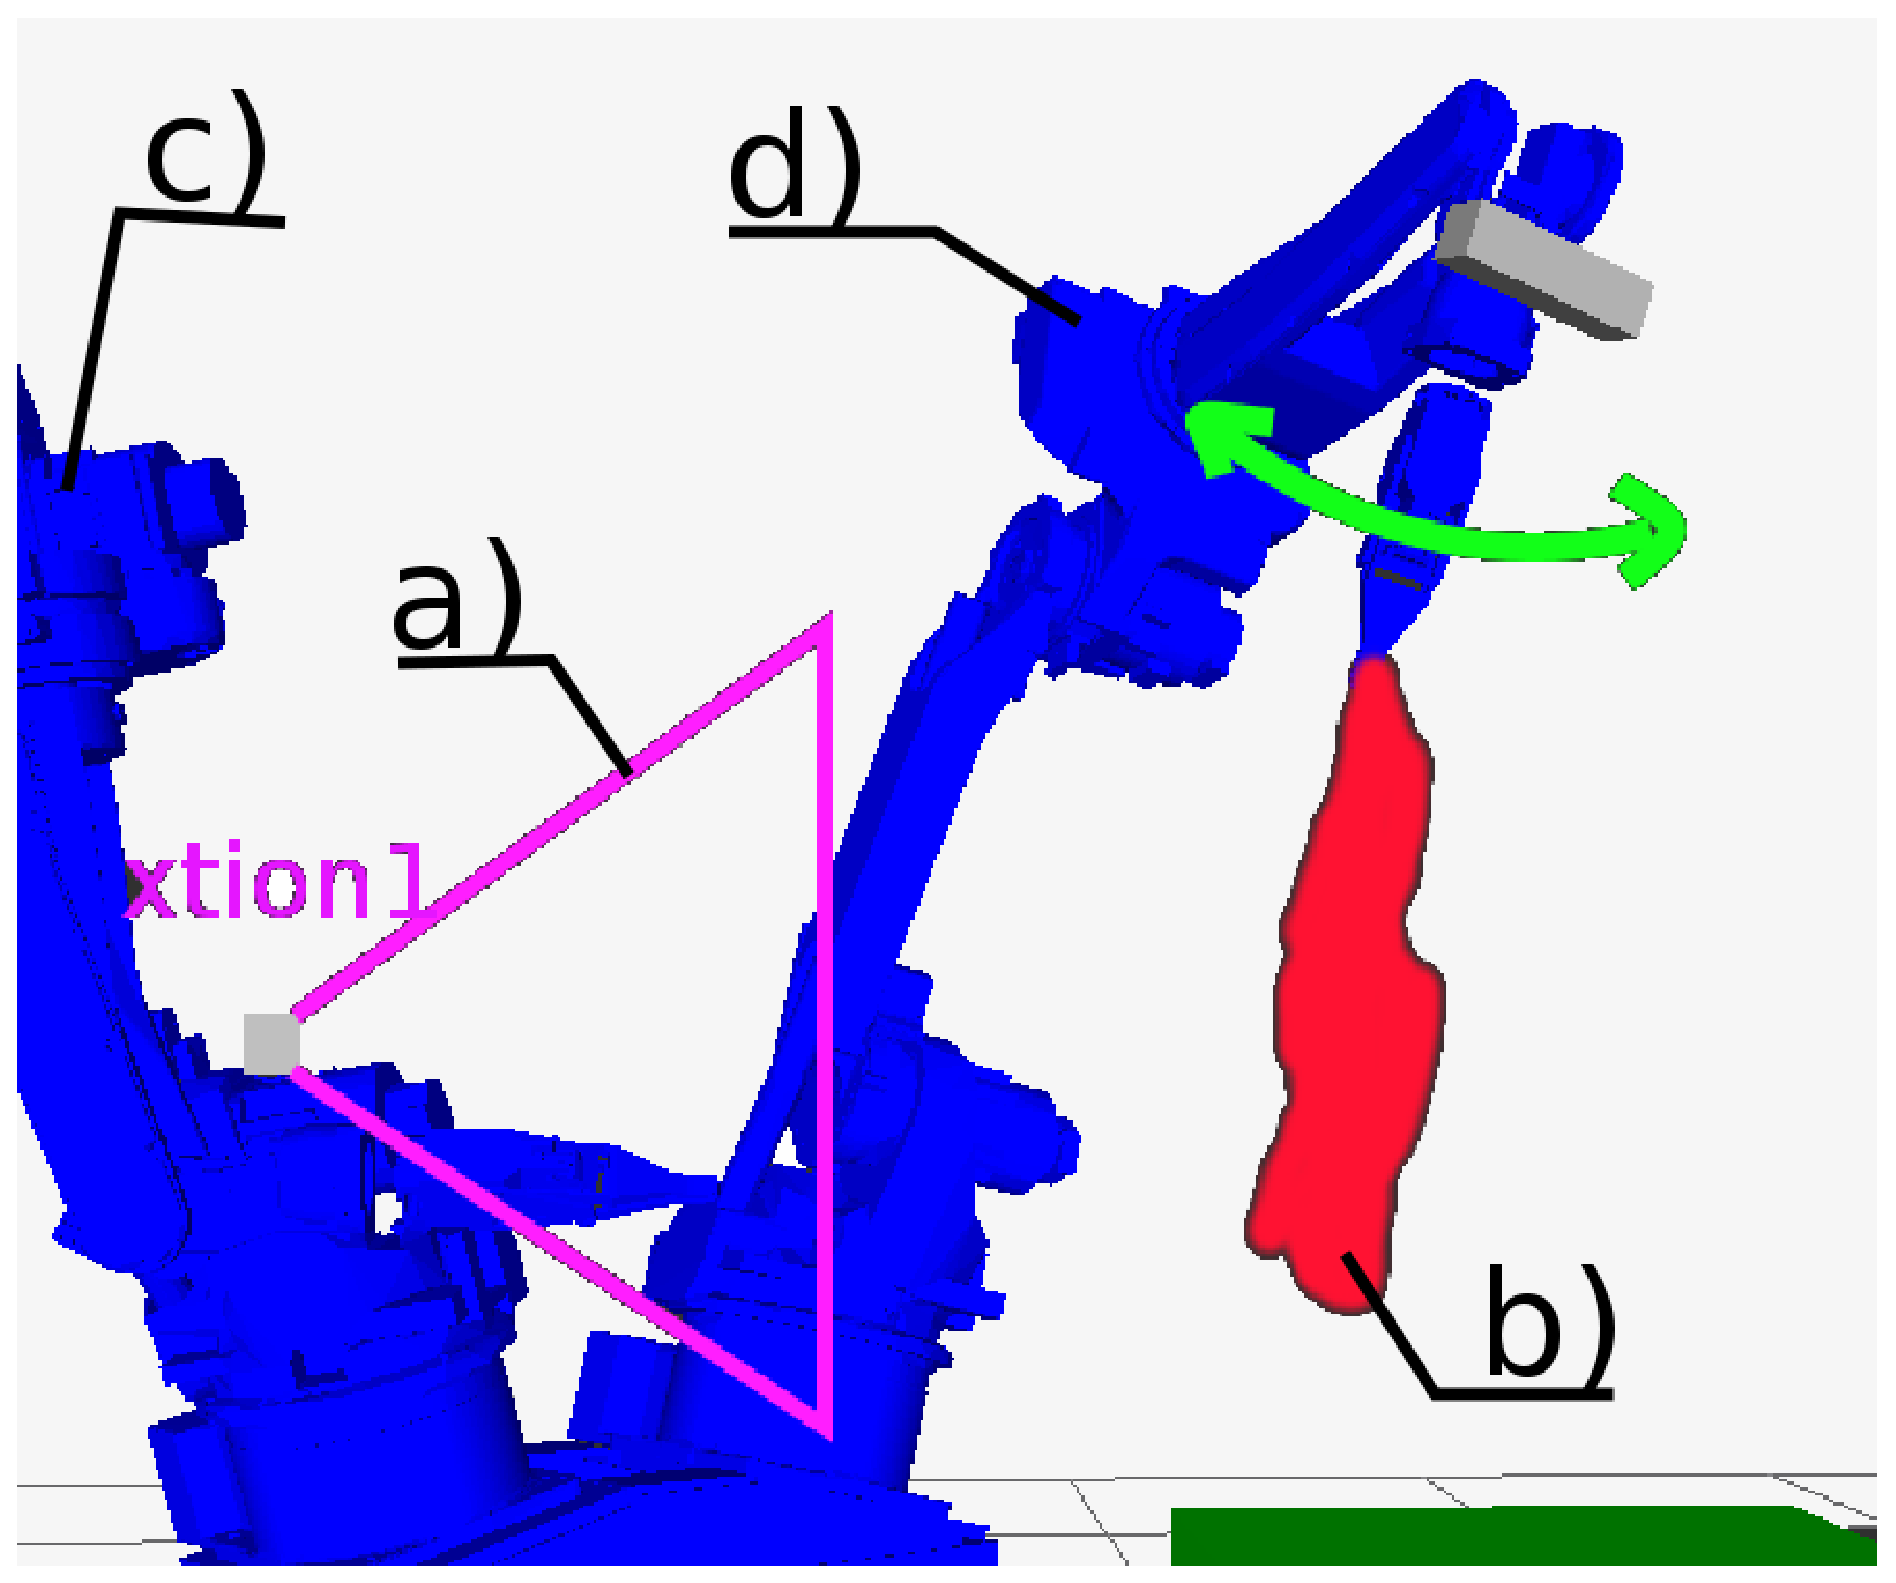
\includegraphics[height=7cm]{pictures/move2.eps}
  	\caption{Nastínění pohybů chapadla s textilií podél optické osy\\
  	a) naznačení zorného pole kamery xtion1, b) textilie, c) paže r1, d) paže r2.}
  	\label{fig:rovnoOptOsy}
\end{figure}



%\noindent Po skončení snímání je možné vyměnit látku a postup zopakovat.\\
%\\
\noindent Přesné polohy a pohyby paží je možné vyčíst ze souboru:\\ \verb|path_to_workspace/clopema_collect_model_data/src/_pos.py|. Pro nahlédnutí do tohoto souboru je nutné splnit předpoklady z kapitoly~\ref{sec:prd}.

%------------------------------------------------------------------------------------
%------------------------------------------------------------------------------------
%------------------------------------------------------------------------------------
%------------------------------------------------------------------------------------
%------------------------------------------------------------------------------------
%------------------------------------------------------------------------------------
%------------------------------------------------------------------------------------
%------------------------------------------------------------------------------------
%------------------------------------------------------------------------------------
%------------------------------------------------------------------------------------
%------------------------------------------------------------------------------------
%------------------------------------------------------------------------------------
%------------------------------------------------------------------------------------
%------------------------------------------------------------------------------------
%------------------------------------------------------------------------------------
%------------------------------------------------------------------------------------

\chapter{Pořízení dat}

\section{Předpoklady}
\label{sec:prd}
\begin{enumerate}

   \item Nainstalovaný ROS Hydro a balíčky CloPeMa dle návodu z Wikipedie projektu~\cite{wikiPack}.
%  \begin{itemize} 
%  
%  	\item \verb|http://clopema.felk.cvut.cz/redmine/projects/clopema/wiki/CloPeMa_Packages|
%  \end{itemize}
  
  \item Stáhnutý archív se zdrojovými kódy \red{Presun na CloPeMu}:
  \begin{itemize}
  	\item \verb|git clone https://github.com/michalneoral/clopema_collect_model_data.git|
  \end{itemize}
  
  \item V balíčku \verb|clopema_collect_model_data| ve složce \verb|src| uprav script \verb|local_options.py| pro místní nastavení počítače. Po otevření v příslušném textovém editoru upravte obsah proměnných pro Vaše umístění. 
  \begin{itemize}
  	\item \verb|pcglocate| pro umístění složky se zdrojovými kódy
  	\item \verb|savefolder| umístění složky, kam se budou ukládat získaná data.
  \end{itemize}
\end{enumerate}


\section{Postup spouštění}
\label{sec:runScript}

\begin{enumerate}
 
  \item Před měřením nastavte omezení rychlosti robota na TEACH-PENDANTu na 10000 dle návodu~\cite{robotConf}. Po měření uveďte nastavení omezení do původního stavu. 
%  	\begin{itemize}
%   		\item \verb|http://clopema.felk.cvut.cz/redmine/projects/clopema/wiki/Robot_configuration|
%   		\item Po měření uveďte do původního stavu.
%  	\end{itemize}
   
  
  \item \label{itm:robOn} Spustíme robota: 
  	\begin{itemize}  
  		\item \verb|roslaunch clopema_launch start_robot.launch|
  	\end{itemize}
  
  \item \label{itm:camOn} Spustíme kameru na paži \verb|r1|:
  	\begin{itemize}
  		\item \verb|roslaunch clopema_launch xtion1.launch|
 	\end{itemize}
  
  \item Poté, co se body \ref{itm:robOn} a \ref{itm:camOn} úspěšně spustí můžeme spustit vlastní skript pro sběr dat:
  	\begin{itemize}
  		\item \verb|rosrun clopema_collect_model_data collect_data.py|
  	\end{itemize}
  
  \item Program je ovládán z příkazové řádky.
  
\end{enumerate}


\section{Ovládání skriptu collect\_data.py pro snímání dat}
\label{sec:program}

\subsection{Popis ovládání}
Skript již máme spuštěn podle návodu v kapitole~\ref{sec:runScript}. Po spuštění se nám zobrazí úvodní menu zobrazené na obrázku \ref{fig:menu}.
Čísla v závorkách \textbf{(číslo)} značí pozici funkce v menu programu. Např.~funkci~\textbf{(4)}~\textit{Open~Gripper} (otevření chapadla) spustíme vepsáním čísla \verb|4| a potvrzením klávesy \verb|Enter|. Obdobně postupujeme při spouštění i dalších funkcí. Pro ukončení programu vepíšeme slovo \verb|stop| a potvrdíme klávesou \verb|Enter|. Program \textbf{nedoporučuji} ukončit stiskem \verb|ctrl+c|.

\begin{figure}[H]
	\centering  	
  	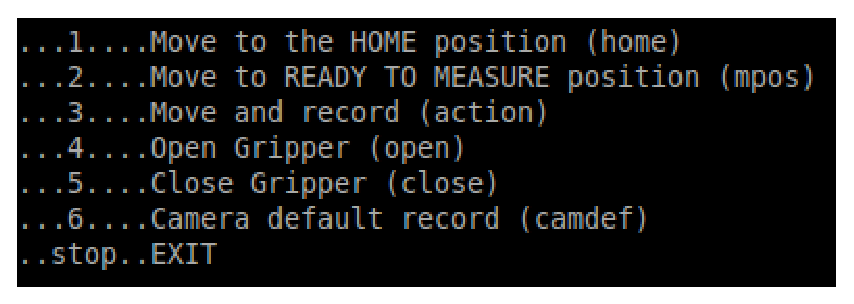
\includegraphics[scale=0.6]{pictures/obrazek3.eps}
  	\caption{Náhled menu skriptu}
  	\label{fig:menu}
\end{figure}

\subsection{Postup pro nasnímání obrazu pro odfiltrování pozadí}
\label{subsec:processFiltrSave}
\begin{enumerate}
  \item Využijeme funkci \textbf{(6)} – \textit{Camera default record} (obrázek \ref{fig:menu}).
\end{enumerate}

\subsection{Postup pořízení dat – manuální vkládání textilie:}
\begin{enumerate}
  \item Umístíme robota do polohy, ve které je připraven k měření \textbf{(2)} - \textit{Move to READY TO MEASURE position} (obrázek \ref{fig:menu}).
  \item Otevřeme chapadlo \textbf{(4)} – \textit{Open Gripper}.
  \item Zavřeme chapadlo \textbf{(5)} – \textit{Close Gripper}. Po stisknutí máme 5 vteřin pro vložení textilie do chapadla než se chapadlo sevře.
  \item Po sevření chapadla ustoupíme do bezpečné vzdálenosti od robota.
  \item Zahájíme měření a záznám \textbf{(3)} - \textit{Move and record}.
  \item Budeme vyzvání k pojmenování souboru. Doporučuji nazývat souboru názvem textilie, případně i pořadovým číslem.
  \item Po schválení názvu souboru bude provedeno měření způsobem, který je popsán v předchozí kapitole \nameref{chap:proveData} (kapitola \ref{chap:proveData}).
  \item Postup 2. až 7. můžeme opakovat pro další měření.
  \item Před ukončením programu můžeme pomocí \textbf{(1)} umístit robota do výchozí polohy.
  \item Program ukončíme pomocí \textbf{(exit)}.
\end{enumerate}

%------------------------------------------------------------------------------------
%------------------------------------------------------------------------------------
%------------------------------------------------------------------------------------
%------------------------------------------------------------------------------------
%------------------------------------------------------------------------------------
%------------------------------------------------------------------------------------
%------------------------------------------------------------------------------------
%------------------------------------------------------------------------------------
%------------------------------------------------------------------------------------
%------------------------------------------------------------------------------------
%------------------------------------------------------------------------------------
%------------------------------------------------------------------------------------
%------------------------------------------------------------------------------------
%------------------------------------------------------------------------------------
%------------------------------------------------------------------------------------
%------------------------------------------------------------------------------------

\chapter{Uložení dat}

\section{Formát dat}
Data se ukládají pomocí rosbag (nástroj ROSu) ve formátu “.bag“ do předem určené složky uložené v souboru \verb|local_options.py| (\verb|path_to_workspace/clopema_collect_model_data/src/local_options.py|).
\\

\section{Témata (topics)}
Z důvodu úspory místa a kapacity přenosového kanálu jsou zaznamenány pouze témata (topics), která jsou uložena v souboru \verb|path_to_workspace/clopema_collect_model_data/matlab/topics/topics.txt|.\\ Pro~tento experiment jsem vybral tyto témata (topics):\\
\\
\indent \indent \indent \verb|/joint_states| \\
\indent \indent \indent \verb|/tf| \\
\indent \indent \indent \verb|/xtion1/depth/camera_info| \\
\indent \indent \indent \verb|/xtion1/depth_registered/camera_info| \\
\indent \indent \indent \verb|/xtion1/projector/camera_info| \\
\indent \indent \indent \verb|/xtion1/rgb/camera_info| \\
\indent \indent \indent \verb|/xtion1/depth/image_raw| \\
\indent \indent \indent \verb|/xtion1/rgb/image_raw |\\
\indent \indent \indent \verb|/xtion1/depth/disparity |\\
%\indent \indent \indent \verb|/xtion1/depth/points|\\

\noindent Seznam témat je možné libovolně měnit. Zaznamenáno je 7 vteřin dat.
%\red{Popsat proč 7 vteřin}
\\

\section{Formát názvu}
\label{sec:nameform}
Zaznamenané soubory jsou ve tvaru: \verb|name_speed_AX.bag|

\begin{itemize}
\item \itab{name}  \tab{vámi zadaný název}
\item \itab{speed} \tab{nastavená rychlost manipulátoru} 
\item \itab{A} \tab{osa, kterou byl vykonán pohyb} \begin{center}
					\verb|R| nebo \verb|B| (obrázek \ref{fig:motomanAxis}).~~~~~~~~~~~~~~~~~~~~~~~~~~~~~~~~~~~~~~~~\end{center}					
\item \itab{X}  \tab{číslo souboru s tématy, která jsou zaznamenána}  
\end{itemize}

%------------------------------------------------------------------------------------
%------------------------------------------------------------------------------------
%------------------------------------------------------------------------------------
%------------------------------------------------------------------------------------
%------------------------------------------------------------------------------------
%------------------------------------------------------------------------------------
%------------------------------------------------------------------------------------
%------------------------------------------------------------------------------------
%------------------------------------------------------------------------------------
%------------------------------------------------------------------------------------
%------------------------------------------------------------------------------------
%------------------------------------------------------------------------------------
%------------------------------------------------------------------------------------
%------------------------------------------------------------------------------------
%------------------------------------------------------------------------------------
%------------------------------------------------------------------------------------


\chapter{Načtení dat pro další zpracování}
\label{chap:matlab}
\section{Předpoklady}
\begin{enumerate}
  \item Stahnutý archív se zdrojovými kódy \red{přesun na CloPeMu}
  \begin{itemize}
  	\item \verb|git clone https://github.com/michalneoral/clopema_collect_model_data.git|
  \end{itemize}
  
  \item Nainstalujte Matlab (odzkoušeno ve verzi 2012b i 2013a).
  \item Nainstalujte toolbox~\cite{toolbox} pro matlab „rosbag“ a přidána cesta pro tento toolbox. %Toolbox je dostupný i s návodem k instalaci na adrese:
%  \begin{itemize}
%     \item \verb|https://github.com/bcharrow/matlab_rosbag|
%  \end{itemize}
  \item Nacházejte se ve složce se zdrojovými kódy pro Matlab.
  \item Soubor \verb|topics/topics.txt| musí být stejný jako v době nahrávání .bag souboru.
  \item Soubor \verb|local_options.m| přizpůsobte vašemu nastavení (blíže popsáno přímo v souboru po otevření souboru v editoru).
\end{enumerate}

\section{Načtení souborů do Matlabu}
\label{sec:loadBag}
\begin{enumerate}
  \item Spusťte skript \verb|startup.m|. Skript připraví prostředí a načte proměnné ze souboru \verb|local_options.m|.
    \begin{itemize}
  	\item \verb|startup|
  \end{itemize}
  \item Pomocí funkce \verb|loadBagFile()| načtěte požadovaný .bag soubor.
	\label{itm:load1}    
    \begin{itemize}
  	\item \verb|msgs = loadBagFile( path_to_bag_files, topics, bagfile)|
    \end{itemize}
    		Vstupy do funkce
        		\begin{itemize}
  			\item \verb|path_to_bag_files| (\textit{řetězec}) - obsahuje umístění složky ve které jsou uloženy .bag soubory.
  			\item \verb|topics| (\textit{matice buněk s řetězci}) - obsahuje názvy témat (topic), která se mají vybrat z .bag souboru pro zpracování.
  			\item \verb|bagfile| (\textit{řetězec}) - název požadovaného .bag souboru. Způsob nazývání souborů byl popsán v kapitole \ref{sec:nameform}.
    			\end{itemize}
    		Výstupy z funkce
        		\begin{itemize}
  			\item \verb|msgs| (\textit{matice buněk}) - obsahuje témata (topic) z požadovaného .bag souboru (data a informace).
    			\end{itemize}
    \item Pomocí funkce \verb|loadBackgroundRGB()| načtěte referenční snímek pro odfiltrování pozadí při snímání RGB kamerou.
	\label{itm:load2} 
    \begin{itemize}
  	\item \verb|rgb_back = loadBackgroundRGB( path_to_bag_files, bagfile_backgroung)|
    \end{itemize}
    		Vstupy do funkce
        		\begin{itemize}
  			\item \verb|path_to_bag_files| (\textit{řetězec}) - obsahuje umístění složky ve které jsou uloženy .bag soubory.
  			\item \verb|bagfile_backgroung| (\textit{řetězec}) - název požadovaného .bag souboru s nasnímaným pozadím. Název pro výchozí souboru je \verb|camera_default_0.bag|.
    			\end{itemize}
    		Výstupy z funkce
        		\begin{itemize}
  			\item \verb|rgb_back| (\textit{matice}) - obsahuje RGB obrázek pozadí ve formátu \textit{double}. Možno zobrazit pomocí \verb|image(rgb_back)|.
    			\end{itemize}
Funkce z bodu \ref{itm:load1} a \ref{itm:load2} lze také spustit pomocí příkazu \verb|loader|.   
\end{enumerate}
%V proměnné \verb|path_to_bag_files| je potřeba mít uloženou cestu k uloženým \verb|*.bag| souborům s daty a v proměnné \verb|topics| je načten soubor \verb|topics.txt| s názvy požadovaných témat (viz. %\verb|startup.m|).\\
%\\
%Načítání souborů spustíte příkazem \verb|loader|, který vypíše soubory v zadané složce (\verb|path_to_bag_files|) a nechá vybrat soubor pro načtení do Matlabu a vypíše informace o souboru. Pro správnou %funkci tohoto skriptu je třeba mít nasnímáno a uloženo „čisté“ pozadí (popsáno v kapitole \textit{Návod na pořízení dat}).\\
%\\
%Tento příkaz dále spustí skript \verb|reader|, který převede soubor .bag na čitelnější strukturu \verb|msgs| (provede rovněž i pro „čisté“ pozadí \verb|msgs_bag|) a předpřipravý RGB obrázek „čistého“ %pozadí - \verb|rgb_back| (takto předpřipravené data lze zobrazovat pomocí \verb|imshow(data)| nebo \verb|image(data)| jako 2D obrazy). \\
%\\
%Příkaz loader dále předpřipraví data z RGB i hloubkové kamery do zásobníku obrazu \verb|front|, která je seřazená tak, aby si obrazy odpovídaly časovými značkami. První řádek obsahuje původní RGB %obrazy, druhý řádek obsahuje RGB obrazy s odfiltrovaným pozadím a třetí řádek obsahuje data z hloubkové kamery v metrech.
%Spolu se strukturou \verb|front| se tvoří i struktura \verb|queue|, jenž v obsahuje tyto údaje:
%
\section{Předzpracování dat}
Jak jsem uvedl v kapitole~\ref{sec:moveArm}~a~\ref{sec:nameform} je záznam pohybu chapadla s látkou rozdělen do dvou souborů. Záznamy končící písmenem \verb|R| jsou určeny pro následné zpracování dat ze senzoru hloubkové mapy a záznamy končící písmenem \verb|B| jsou určeny pro zpracování RGB snímků (písmena označují, kterou osou je na daném záznamu pohybováno pro vytvoření pohybu látky). Další zpracování se tedy bude lišit podle toho, zda chceme extrahovat matematické příznaky látky z hloubkové mapy~(\ref{sec:procDepth}) nebo z RGB snímků~(\ref{sec:procRgb}). 

\section{Zpracování RGB dat}
\label{sec:procRgb}
Z kapitoly \ref{sec:loadBag} již máme připravená data v matici buněk \verb|msgs|. Z této matice buněk extrahujeme pouze data, která se týkají RGB obrázku a vytvoříme si posloupnost nasnímaných RGB obrázků s časy ve kterých byly zachyceny. Posloupnost vytvoříme pomocí funkce \verb|makeFrontOfRGB()|.
\begin{itemize}
  	\item \verb|frontOfRGB = makeFrontOfRGB( msgs )|

    		Vstupy do funkce
        		\begin{itemize}
  			\item \verb|msgs| (\textit{matice buněk}) - je výstup z funkce popsané v~\ref{sec:loadBag}.\ref{itm:load1}.
    			\end{itemize}
    		Výstupy z funkce
        		\begin{itemize}
  			\item \verb|frontOfRGB| (\textit{matice buněk}) - obsahuje posloupnost RGB obrázků (\textit{double} 640x480x3) a čas zachycení obrázku v \textit{s} (\textit{double}). 
    			\end{itemize}
    \end{itemize}

\red{Zde vložit obrázky - příklad zobrazení RGB obrázku}

\subsection{Filtrování RGB snímků pomocí referenčního snímku}
\label{subsec:matfiltr}
Na RGB snímcích jsou mi pohybující se látku i věci nedůležité pro experiment (stále pozadí, části manipulátoru...). Tyto části obrazu je potřeba odstranit. Odstraněním části obrazu mimo pohybující se látku nám pomůže snáze sledovat pohybující se siluetu látky. Látku odstraníme pomocí referenčního snímku, jehož způsob pořízení jsme si uvedli v kapitolách~\ref{subsec:refRGB}~a~\ref{subsec:processFiltrSave}. Funkce \verb|filtrReferenceFrame()| slouží k tomuto filtrování.
\begin{itemize}
  	\item \verb|[filtredFrontOfRGB, maskFrontOfRGB] =|\\ \verb|filtrReferenceFrame(frontOfRGB,referenceFrame,sizeMorpMask)|\\
\\
    		Vstupy do funkce
        		\begin{itemize}
  			\item \verb|frontOfRGB| (\textit{matice buněk}) - matice buňek obsahující obrázky.
  			\item \verb|referenceFrame| (\textit{matice double} 640x480x3) - obsahuje referenční snímek.
  			\item \verb|sizeMorpMask| (\textit{integer}) - \textit{nepovinný} parametr, kterým se nastavuje velikost masky pro morfologickou  operaci "opening"\cite{hlavacOpen}.
    			\end{itemize}
    		Výstupy z funkce
        		\begin{itemize}
        		\item \verb|filtredFrontOfRGB| (\textit{matice buněk}) - obsahuje filtrované obrazy RGB a časovou značku původních snímků.
  			\item \verb|maskFrontOfRGB| (\textit{matice buněk}) - obsahuje filtry obrazů RGB a časovou značku původních snímků.
    			\end{itemize}
    \end{itemize}

\red{Zde vložit obrázky - příklad zobrazení vyfiltrovaného RGB obrázku}





\subsection{Nalezení kostry obrazů}

\red{Zde vložit popis}\\

\red{Zde vložit obrázky - příklad zobrazení získané kostry z vyfiltrovaného RGB obrázku}





\subsection{Získání matematických příznaků látky z kostry obrazů v čase}

\red{Zde vložit popis}\\

\red{Zde vložit ukázku získaných dat}


%-HHHHHHHHHHHHHHHHHHHHHHHHHHHHHHHHHHHHHHHHHHHHHHHHHHHHHHHHHHHHHHHHHHHHHHHHHHHHHHHHHHHHHHHHHHHHHHHHHHHHHHHHHHHHHHHHHHHHHHHHHHHHHHHHHHHHHHHHHHHHHHHHHHHHHHHHHHHHHHHHH-
%-HHHHHHHHHHHHHHHHHHHHHHHHHHHHHHHHHHHHHHHHHHHHHHHHHHHHHHHHHHHHHHHHHHHHHHHHHHHHHHHHHHHHHHHHHHHHHHHHHHHHHHHHHHHHHHHHHHHHHHHHHHHHHHHHHHHHHHHHHHHHHHHHHHHHHHHHHHHHHHHHH-
%-HHHHHHHHHHHHHHHHHHHHHHHHHHHHHHHHHHHHHHHHHHHHHHHHHHHHHHHHHHHHHHHHHHHHHHHHHHHHHHHHHHHHHHHHHHHHHHHHHHHHHHHHHHHHHHHHHHHHHHHHHHHHHHHHHHHHHHHHHHHHHHHHHHHHHHHHHHHHHHHHH-
%-HHHHHHHHHHHHHHHHHHHHHHHHHHHHHHHHHHHHHHHHHHHHHHHHHHHHHHHHHHHHHHHHHHHHHHHHHHHHHHHHHHHHHHHHHHHHHHHHHHHHHHHHHHHHHHHHHHHHHHHHHHHHHHHHHHHHHHHHHHHHHHHHHHHHHHHHHHHHHHHHH-

\section{Zpracování dat ze senzoru hloubkové mapy}
\label{sec:procDepth}
Z kapitoly \ref{sec:loadBag} již máme připravená data v matici buněk \verb|msgs|. Z této matice buněk extrahujeme pouze data, která se týkají hloubkové mapy a vytvoříme si posloupnost nasnímaných hloubkových map s časy ve kterých byly zachyceny. Posloupnost vytvoříme pomocí funkce \verb|makeFrontOfDepth()|.
\begin{itemize}
  	\item \verb|frontOfDepth = makeFrontOfDepth( msgs )|

    		Vstupy do funkce
        		\begin{itemize}
  			\item \verb|msgs| (\textit{matice buněk}) - je výstup z funkce popsané v~\ref{sec:loadBag}.\ref{itm:load1}.
    			\end{itemize}
    		Výstupy z funkce
        		\begin{itemize}
  			\item \verb|frontOfDepth| (\textit{matice buněk}) - obsahuje posloupnost hloubkových map (\textit{double} 640x480) a čas zachycení mapy v \textit{s} (\textit{double}). 
    			\end{itemize}
    \end{itemize}

\red{Zde vložit obrázky - příklad zobrazení hloubkové mapy zachycené senzorem}




\subsection{Filtrování hloubkové mapy dle vzdálenosti zájmové oblasti}

\red{Zde vložit popis}\\

\red{Zde vložit obrázky - odfiltrování nežádoucích vzdáleností}




\subsection{Nalezení bodů (oblastí) na povrchu látky}

\red{Zde vložit popis}\\

\red{Zde vložit obrázky - příklad nalezených bodů}




\subsection{Získání matematických příznaků látky ze vzdáleností bodů v čase}

\red{Zde vložit popis}\\

\red{Zde vložit ukázku získaných dat}

%$$\begin{bmatrix}
%\verb|pořad. číslo hloubkového snímku| & \verb|čas od začátku měření| & \verb|pořad. číslo tématu v msgs| \\
%  \verb|pořad. číslo rgb snímku| & \verb|časový rozdíl mezi snímky| & \verb|pořad. číslo tématu v msgs|
%\end{bmatrix} $$\\
%\\



%------------------------------------------------------------------------------------
%------------------------------------------------------------------------------------
%------------------------------------------------------------------------------------
%------------------------------------------------------------------------------------

%\chapter{Provedení experimentu}

%------------------------------------------------------------------------------------
%------------------------------------------------------------------------------------
%------------------------------------------------------------------------------------
%------------------------------------------------------------------------------------
\newcounter{lit}
\begin{thebibliography}{00}

\bibitem[\arabic{lit}]{version} Neoral Michal:
    \emph{Aktuální verze tohoto návodu} [online]. \\
    Dostupné z: \verb|https://github.com/michalneoral/collect_data_documentation/|\\
	\verb|raw/master/manual_collect_data(cze).pdf|

\stepcounter{lit}  
  \bibitem[\arabic{lit}]{projekt} CloPeMa:
    \emph{Stránky projektu CLoPeMa} [online]. [cit. 2014-02-02].\\
    Dostupné z: \verb|http://clopemaweb.felk.cvut.cz/|

\stepcounter{lit}
  \bibitem[\arabic{lit}]{wiki} CloPeMa:
    \emph{Wikipedie projektu CLoPeMa} [online]. [cit. 2014-02-02].\\
    Dostupné z: \verb|http://clopema.felk.cvut.cz/redmine/projects/clopema/wiki|
    
\stepcounter{lit}
  \bibitem[\arabic{lit}]{wikiDes} CloPeMa:
    \emph{Wikipedie projektu CLoPeMa - technické záležitosti} [online]. [cit. 2014-02-02].\\
    Dostupné z: \verb|http://clopema.felk.cvut.cz/redmine/projects/clopema/wiki/Technical_Stuff|
    
\stepcounter{lit}
  \bibitem[\arabic{lit}]{wikiPack} CloPeMa:
    \emph{Wikipedie projektu CLoPeMa - Balíčky projektu CloPeMa} [online]. [cit. 2014-02-02].\\
    Dostupné z: \verb|http://clopema.felk.cvut.cz/redmine/projects/clopema/wiki/CloPeMa_Packages|    

\stepcounter{lit}
  \bibitem[\arabic{lit}]{robotConf} CloPeMa:
    \emph{Wikipedie projektu CLoPeMa - Nastavení omezení rychlosti} [online]. [cit. 2014-02-02].\\
    Dostupné z: \verb|http://clopema.felk.cvut.cz/redmine/projects/clopema/wiki/Robot_configuration|  

\stepcounter{lit}
  \bibitem[\arabic{lit}]{toolbox} Ben Charrow:
    \emph{Toolbox pro Matlab určený ke čtení rosbag souborů} [online]. [cit. 2014-02-02].\\
    Dostupné z: \verb|http://clopema.felk.cvut.cz/redmine/projects/clopema/wiki/Robot_configuration|  

\verb|https://github.com/bcharrow/matlab_rosbag|

\stepcounter{lit}    
  \bibitem[\arabic{lit}]{homesim} Neovision:
    \emph{Industrial Vision System} [online]. [cit. 2013-11-12].\\
    Dostupné z: \verb|http://www.neovision.cz/cz/sols/clopema.html|    

\stepcounter{lit}  
  \bibitem[\arabic{lit}]{gripperPic} Václav Jahoda:
    \emph{CloPeMa} [online]. [cit. 2013-11-27].\\
    Technický výkres \verb|12010_00_04_Robot.pdf| - UPRAVENO\\
    Dostupné z: \verb|clopema.felk.cvut.cz/redmine/attachments/download/121/12010_00_04_Robot.pdf|    

\stepcounter{lit}    
  \bibitem[\arabic{lit}]{motoman} Motoman:
    \emph{YASKAWA Electric Corporation} [online]. [cit. 2013-11-27].\\
    Technický výkres robotického ramena MA1400 - UPRAVENO
    Dostupné z: \verb|http://www.motoman.com.tr/index.php?eID=tx_nawsecuredl&u=0&file=uploads/|\\
    \verb|tx_catalogrobot/MA1400_15.pdf&t=1385654785&hash=ba1cae139705f02080bcf1f7c60f741c8df7434c|
    
\stepcounter{lit}    
  \bibitem[\arabic{lit}]{hlavacOpen} ŠONKA, Milan, Václav HLAVÁČ.
    \emph{Image processing, analysis, and machine vision: a MATLAB companion.} 3rd ed. Toronto: Thomson, 2008. STRANU DODÁM, ISBN 978-0-495-08252-1. 

\end{thebibliography}

\end{document}

